% Зачем: Изменение надписи для списка литературы
% Почему: Пункт 2.8.1 Требований по оформлению пояснительной записки.
\renewcommand{\bibsection}{\sectioncentered*{Cписок использованных источников}}
\phantomsection\pagebreak % исправляет нумерацию в документе и исправляет гиперссылки в pdf
\addcontentsline{toc}{section}{Cписок использованных источников}



% Зачем: включить в список литературы все источники из базы (даже если на них нет ссылок в тексте).
% \nocite{*}

% Зачем: Печать списка литературы. База данных литературы - файл bibliography_database.bib
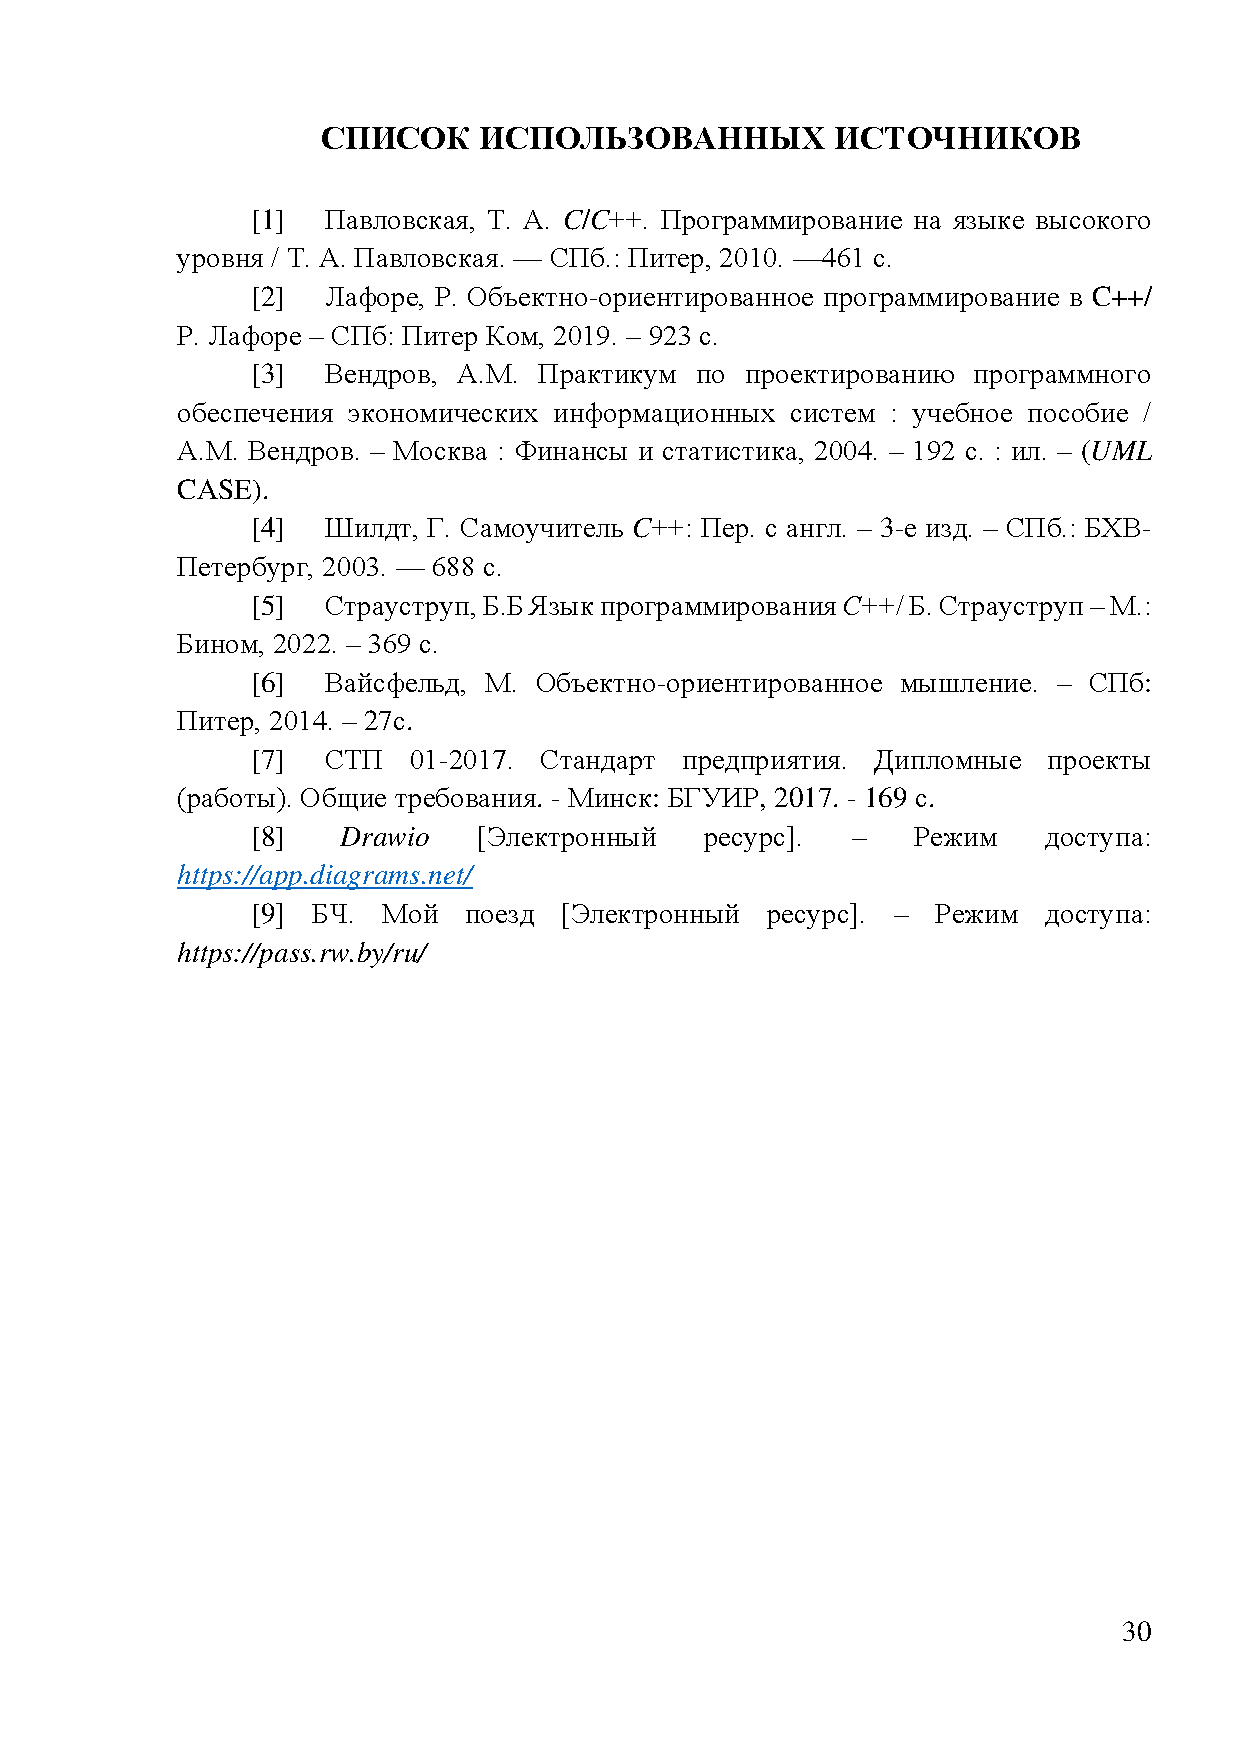
\includepdf[pages = 1]{30-44.pdf}